\documentclass[conference]{IEEEtran}

\usepackage[utf8]{inputenc}
\usepackage[T1]{fontenc}
\usepackage[spanish]{babel}
\usepackage{amsmath,amssymb}
\usepackage{graphicx}
\usepackage{booktabs,array}
\usepackage{siunitx}
\usepackage{circuitikz}
\usepackage{url}
\usetikzlibrary{calc}

\graphicspath{
    {./}{./Figuras/}
}

\sisetup{mode=math,group-separator={\,},group-minimum-digits=5,output-decimal-marker={.}}
\addto\captionsspanish{\renewcommand{\tablename}{Tabla}\renewcommand{\figurename}{Fig.}}
\AtBeginDocument{\renewcommand{\tablename}{Tabla}\renewcommand{\figurename}{Fig.}\ifdefined\decimalpoint\decimalpoint\fi}
\renewcommand{\tablename}{Tabla}

\newcommand{\gm}{g_m}
\newcommand{\kn}{k_n}
\newcommand{\Vov}{V_{OV}}
\newcommand{\Vtp}{V_t'}
\newcommand{\knp}{k_n'}

\begin{document}

\title{Caracterización de un MOSFET 2N7000 y diseño de un amplificador de fuente común: pre-informe de la Práctica 4}

\author{
\IEEEauthorblockN{Juan José Tobar Álvarez\IEEEauthorrefmark{1},
Nombre Apellido 2\IEEEauthorrefmark{1},
Nombre Apellido 3\IEEEauthorrefmark{1}}
\IEEEauthorblockA{\IEEEauthorrefmark{1}Departamento de Ingeniería Eléctrica y Electrónica, Universidad Nacional de Colombia, Bogotá, Colombia\\
jutobara@unal.edu.co, correo2@unal.edu.co, correo3@unal.edu.co}
}

\maketitle

%==================================================================
\section{Introducción/Justificación}
%==================================================================

\subsection{Introducción}
En un MOSFET de canal n de enriquecimiento, como el 2N7000, el canal solo se forma cuando la tensión compuerta--fuente $V_{GS}$ supera la tensión umbral $V_t$; según $V_{GS}$ y la tensión drenador--fuente $V_{DS}$, el dispositivo opera en corte, triodo o saturación \cite{sedra}. La saturación es la región de amplificación, pues allí la corriente de drenador $I_D$ queda controlada por $V_{GS}$ casi sin depender de $V_{DS}$. El análisis DC se realiza con la ley de Ohm y las leyes de Kirchhoff, y el análisis AC con el modelo de pequeña señal, caracterizado por la transconductancia $\gm$ \cite{sedra}.

\textbf{Objetivo general.} Caracterizar el MOSFET 2N7000 y diseñar un amplificador de fuente común, verificándolo mediante simulación.

\textbf{Objetivos específicos.} (i) Determinar $V_t$ y $\kn$ y obtener las curvas $I_D$--$V_{DS}$; (ii) calcular el punto de polarización, $A_v$, $Z_{in}$, $Z_{out}$ y los límites de pequeña señal; (iii) comparar teoría y simulación mediante el error relativo porcentual.

\subsection{Justificación}
El 2N7000 es un MOSFET DMOS vertical de canal n (60 V, 200 mA, encapsulado TO-92) pensado para amplificación, conmutación y control de motores \cite{datasheet}. Su estructura y los principios de polarización que se practican aparecen en aplicaciones de alta exigencia. En el sector aeroespacial, los MOSFET DMOS verticales han sido el dispositivo de conmutación más utilizado en los sistemas de potencia espaciales de la NASA \cite{shea}, y el Centro de Vuelo Espacial Goddard mantiene actividades de aseguramiento de dureza a la radiación para estos transistores \cite{lauenstein}. En la industria médica, los amplificadores CMOS forman el extremo frontal analógico de los sistemas portátiles de adquisición de señales biomédicas \cite{kao}. En telecomunicaciones, los MOSFET LDMOS se emplean en los amplificadores de potencia de las estaciones base celulares \cite{litwin}. La práctica enseña a extraer $V_t$ y $\kn$ de un dispositivo real y muestra cómo la polarización fija la ganancia y las impedancias.

%==================================================================
\section{Cálculos}
%==================================================================

\subsection{Parámetros del 2N7000 según la hoja de datos}
En la Tabla~\ref{tab:datasheet} se resumen los parámetros pedidos en la guía \cite{datasheet}: los límites de tensión y de corriente acotan el punto de operación, y el amplio rango de $V_{GS(th)}$ (0.8 a 3 V) indica que $V_t$ debe medirse en cada ejemplar.

\begin{table}[htbp]
\centering
\caption{Parámetros del 2N7000 a $T_A=\SI{25}{\celsius}$ \cite{datasheet}.}
\label{tab:datasheet}
\scriptsize
\renewcommand{\arraystretch}{1.1}
\begin{tabular}{@{}>{\raggedright\arraybackslash}p{3.0cm}>{\raggedright\arraybackslash}p{1.9cm}>{\raggedright\arraybackslash}p{2.6cm}@{}}
\toprule
Parámetro (símbolo) & Valor & Condición \\
\midrule
Ruptura drenador--fuente ($BV_{DSS}$) & 60 V (mín.) & $V_{GS}=\SI{0}{V}$, $I_D=\SI{10}{\micro A}$ \\
Tensión compuerta--fuente ($V_{GS,max}$, $V_{GS,min}$) & $+30$ V, $-30$ V & límite absoluto \\
Alimentación usada ($V_{DD}$, $V_{SS}$) & 10 V, 0 V & $V_{DD}<BV_{DSS}$ \\
Tensión umbral ($V_{GS(th)}$) & 0.8 a 3 V & $V_{GS}=V_{DS}$, $I_D=\SI{1}{mA}$ \\
Corriente de drenador ($I_{D,max}$) & 200 mA & $T_C=\SI{25}{\celsius}$ \\
Potencia disipada ($P_D$) & 1 W & $T_C=\SI{25}{\celsius}$ \\
Resistencia en conducción ($R_{DS(on)}$) & 5.3 $\Omega$ (máx.) & $V_{GS}=\SI{4.5}{V}$ \\
\bottomrule
\end{tabular}
\end{table}

\subsection{Modelo del MOSFET y regiones de operación}
Despreciando la modulación de la longitud del canal, el transistor está en triodo si $V_{DS}<V_{GS}-V_t$, donde se comporta como una resistencia controlada por $V_{GS}$, y en saturación si $V_{DS}\ge V_{GS}-V_t$, donde la corriente es \cite{sedra}
\begin{equation}
I_D=\frac{\kn}{2}\,(V_{GS}-V_t)^2,
\label{eq:sat}
\end{equation}
con $\kn=\mu_n C_{ox}(W/L)$ el parámetro de transconductancia y $\Vov=V_{GS}-V_t$ la tensión de sobreimpulso. La \eqref{eq:sat} describe la saturación, la región de interés para amplificar. En el circuito de la Fig.~\ref{fig:circ_car}(a) la compuerta está unida al drenador ($V_{DS}=V_{GS}$) y, como $V_t>0$, el transistor está en saturación para cualquier $R_1$. Por la ley de Kirchhoff de tensiones,
\begin{equation}
V_{GS}=V_1-I_D R_1,
\label{eq:kvl_car}
\end{equation}
y al variar $R_1$ se recorren distintos pares ($V_{GS}$, $I_D$).

\subsection{Extracción de $V_t$ y $\kn$}
Tomando la raíz cuadrada de la \eqref{eq:sat} se obtiene
\begin{equation}
\sqrt{I_D}=\sqrt{\frac{\kn}{2}}\,(V_{GS}-V_t),
\label{eq:raiz}
\end{equation}
una recta $\sqrt{I_D}=m\,V_{GS}+b$ con pendiente $m=\sqrt{\kn/2}$. Su intercepto con el eje $V_{GS}$ y el valor de $\kn$ son
\begin{equation}
V_t=-\frac{b}{m},\qquad \kn=2m^2.
\label{eq:vt_kn}
\end{equation}
Con los 91 pares ($V_{GS}$, $I_D$) de la Sec.~\ref{sec:sim_car} ($R_1$ de 1 a \SI{10}{k\ohm} en pasos de \SI{100}{\ohm}), el ajuste por mínimos cuadrados de $\sqrt{I_D}$ (A$^{1/2}$) contra $V_{GS}$ (V) es
\begin{equation}
\sqrt{I_D}=0.1891\,V_{GS}-0.2829,\qquad R^2=0.9932,
\label{eq:recta}
\end{equation}
de donde $V_t=\SI{1.496}{V}$ y $\kn=\SI{71.52}{mA/V^2}$ mediante la \eqref{eq:vt_kn}. La guía propone verificar $\kn$ con un solo par de puntos:
\begin{equation}
\kn=\frac{2I_D}{(V_{GS}-V_t)^2}.
\label{eq:kn_punto}
\end{equation}
Para $R_1=\SI{5}{k\ohm}$ ($V_{GS}=\SI{1.6366}{V}$, $I_D=\SI{0.6727}{mA}$) la \eqref{eq:kn_punto} da $\kn=\SI{68.23}{mA/V^2}$, que difiere \SI{4.59}{\percent} del valor del ajuste.

\subsection{Circuito para las curvas características}
Para obtener en una sola simulación la familia de curvas $I_D$--$V_{DS}$ se emplea el circuito de la Fig.~\ref{fig:circ_car}(b), con $V_1=V_{GS}$ en la compuerta y $V_2=V_{DS}$ en el drenador. Se barre $V_2$ de 0 a 10 V y, de forma anidada, $V_1$ de 2 a 4 V en pasos de 0.5 V, todos mayores que $V_t$. La frontera entre triodo y saturación es
\begin{equation}
V_{DS}=V_{GS}-V_t,
\label{eq:frontera}
\end{equation}
es decir, $V_{DS}=\SI{0.504}{V}$ para $V_{GS}=\SI{2}{V}$ y \SI{2.504}{V} para $V_{GS}=\SI{4}{V}$.

\begin{figure}[htbp]
\centering
\begin{minipage}[b]{0.47\columnwidth}
\centering
\resizebox{\linewidth}{!}{%
\begin{circuitikz}
\node[nmos] (M) at (2,0) {};
\draw (M.S) -- ++(0,-0.4) coordinate(GN) node[ground]{};
\draw (M.D) to[short,*-] ++(0,0.6) coordinate(N);
\draw (M.G) -- ++(-0.5,0) |- (N);
\draw (N) to[R=$R_1$] ($(N)+(0,1.8)$) coordinate(T);
\draw (T) -- (-0.6,0 |- T) to[V,l_=$V_1$] (-0.6,-1.2) node[ground]{};
\end{circuitikz}}\\[2pt]
{\footnotesize (a)}
\end{minipage}\hfill
\begin{minipage}[b]{0.47\columnwidth}
\centering
\resizebox{\linewidth}{!}{%
\begin{circuitikz}
\node[nmos] (M) at (2,0) {};
\draw (M.S) -- (M.S |- 0,-1.8) node[ground]{};
\draw (M.G) -- ++(-0.4,0) coordinate(Gg) to[V,l_=$V_1$] (Gg |- 0,-1.8) node[ground]{};
\draw (M.D) to[short,*-] ++(0,0.5) coordinate(Dt) -- (3.4,0 |- Dt) to[V,l=$V_2$] (3.4,-1.8) node[ground]{};
\end{circuitikz}}\\[2pt]
{\footnotesize (b)}
\end{minipage}
\caption{Circuitos de caracterización: (a) diodo conectado para extraer $V_t$ y $\kn$; (b) barrido doble para la familia de curvas $I_D$--$V_{DS}$.}
\label{fig:circ_car}
\end{figure}

\subsection{Parámetros en la zona de operación}
La recta de la \eqref{eq:recta} se obtuvo con $V_{GS}$ entre \SI{1.59}{V} y \SI{1.78}{V}, cerca del umbral, pero el amplificador opera con $V_{GS}\approx\SI{2}{V}$ e $I_D\approx\SI{10}{mA}$. Por ello se repite el ajuste de la \eqref{eq:raiz} con las corrientes de saturación de la Fig.~\ref{fig:curvas} para $V_{GS}$ de 2, 2.5 y 3 V (Tabla~\ref{tab:isat}), lo que con la \eqref{eq:vt_kn} y $m'=\SI{0.2627}{A^{1/2}/V}$ da los parámetros de operación
\begin{equation}
\Vtp=\SI{1.561}{V},\qquad \knp=2m'^2=\SI{138.1}{mA/V^2},
\label{eq:param_op}
\end{equation}
que se usan en el diseño del amplificador (su ventaja se cuantifica en la Sec.~\ref{sec:an_curvas}).

\subsection{Diseño del amplificador de fuente común}
Se diseña el amplificador de la Fig.~\ref{fig:cs} con los parámetros de la Tabla~\ref{tab:param_cs}, con generador ideal ($R_{sig}=\SI{0}{\ohm}$), $r_o\rightarrow\infty$ y los parámetros de operación de la \eqref{eq:param_op}. Los requisitos son saturación y $|v_{out}|\approx 5\,|v_{in}|$: $R_{G1}$ y $R_{G2}$ fijan $I_D\approx\SI{10.8}{mA}$, con lo que $\gm\approx\SI{54.5}{mS}$ (\eqref{eq:gm}) y $|A_v|=\gm(R_D\parallel R_L)\approx 5$ (\eqref{eq:Av}).

\begin{table}[htbp]
\centering
\caption{Parámetros asumidos para el amplificador de fuente común.}
\label{tab:param_cs}
\scriptsize
\renewcommand{\arraystretch}{1.1}
\begin{tabular}{@{}lllll@{}}
\toprule
$V_{DD}$ & $R_{G1}$ & $R_{G2}$ & $R_D$ & $R_S$ \\
\midrule
10 V & 180 k$\Omega$ & 100 k$\Omega$ & 90 $\Omega$ & 150 $\Omega$ \\
\midrule
$R_L$ & $C_1=C_2=C_S$ & $\hat v_{in}$ & $f$ & $R_{sig}$ \\
\midrule
10 k$\Omega$ & 10 $\mu$F & 50 mV (100 mV$_{pp}$) & 10 kHz & 0 $\Omega$ \\
\bottomrule
\end{tabular}
\end{table}

\begin{figure}[htbp]
\centering
\resizebox{0.8\columnwidth}{!}{%
\begin{circuitikz}
\node[nmos] (M) at (0,0) {};
\draw (M.G) -- ++(-0.5,0) coordinate(Gn);
\draw (Gn) to[R=$R_{G1}$,*-] ($(Gn)+(0,2.2)$) -- ++(0,0.3) node[vcc]{$V_{DD}$};
\draw (Gn) to[R=$R_{G2}$,*-] ($(Gn)+(0,-2.2)$) node[ground]{};
\draw (Gn) to[C=$C_1$,*-o] ($(Gn)+(-2,0)$) node[left]{$v_{in}$};
\draw (M.D) to[R=$R_D$,*-] ($(M.D)+(0,2.2)$) -- ++(0,0.3) node[vcc]{$V_{DD}$};
\draw (M.D) to[C=$C_2$] ($(M.D)+(2.8,0)$) coordinate(Out) to[short,*-o] ($(Out)+(0.7,0)$) node[right]{$v_{out}$};
\draw (Out) to[R=$R_L$] ($(Out)+(0,-3.4)$) node[ground]{};
\draw (M.S) to[short,*-] ++(0,-0.3) coordinate(S1) to[R,l_=$R_S$] ($(S1)+(0,-1.9)$) node[ground]{};
\draw (S1) -- ++(1.3,0) to[C=$C_S$] ++(0,-1.9) node[ground]{};
\end{circuitikz}}
\caption{Amplificador de fuente común diseñado.}
\label{fig:cs}
\end{figure}

\paragraph{Análisis DC.} Con $I_G=0$, el divisor de la compuerta equivale a una fuente de Thévenin
\begin{equation}
\begin{gathered}
V_G=V_{DD}\frac{R_{G2}}{R_{G1}+R_{G2}}=\SI{3.571}{V},\\
R_G=R_{G1}\parallel R_{G2}=\SI{64.29}{k\ohm},
\end{gathered}
\end{equation}
que fija la tensión de compuerta. Con la \eqref{eq:thev}, la malla compuerta--fuente da $V_G=\Vtp+\Vov+I_DR_S$ y, al sustituir $I_D=\tfrac{\knp}{2}\Vov^2$ de la \eqref{eq:sat}, resulta una cuadrática en $\Vov$ cuya raíz positiva es
\begin{equation}
\Vov=\frac{-1+\sqrt{1+2\knp R_S\,(V_G-\Vtp)}}{\knp R_S}.
\label{eq:vov}
\end{equation}
Con la \eqref{eq:vov} y los valores de la \eqref{eq:param_op} se obtiene $\Vov=\SI{0.395}{V}$, $I_D=\tfrac{\knp}{2}\Vov^2=\SI{10.77}{mA}$ y $V_{GS}=\SI{1.956}{V}$. Las demás tensiones se calculan con
\begin{equation}
V_S=I_DR_S,\quad V_D=V_{DD}-I_DR_D,\quad V_{DS}=V_D-V_S,
\label{eq:vds}
\end{equation}
que dan $V_S=\SI{1.616}{V}$, $V_D=\SI{9.031}{V}$ y $V_{DS}=\SI{7.415}{V}$. Como $V_{DS}$ de la \eqref{eq:vds} cumple $V_{DS}\ge\Vov$, el transistor opera en saturación, y $I_D<I_{D,max}$ y $P=V_{DS}I_D=\SI{79.9}{mW}<\SI{1}{W}$ respetan la Tabla~\ref{tab:datasheet}.

\paragraph{Análisis AC.} A 10 kHz los capacitores son cortocircuitos y las fuentes DC son tierra de señal. En el modelo de pequeña señal, la transconductancia es
\begin{equation}
\gm=\knp\Vov=\sqrt{2\knp I_D}=\SI{54.54}{mS},
\label{eq:gm}
\end{equation}
y la ganancia de voltaje, con $R_D\parallel R_L=\SI{89.20}{\ohm}$, es
\begin{equation}
A_v=\frac{v_{out}}{v_{in}}=-\gm\,(R_D\parallel R_L)=-4.86\ \text{V/V}.
\label{eq:Av}
\end{equation}
El signo negativo indica inversión de fase y la amplitud de salida esperada es $4.86\times\SI{50}{mV}=\SI{243}{mV}$. Las impedancias de entrada y de salida son
\begin{equation}
Z_{in}=R_{G1}\parallel R_{G2}=\SI{64.29}{k\ohm},\qquad Z_{out}=R_D\parallel r_o=\SI{90}{\ohm},
\label{eq:zin_zout}
\end{equation}
pues la compuerta no consume corriente y $r_o\rightarrow\infty$. Que los capacitores sean cortocircuitos se verifica con la frecuencia de corte de cada uno,
\begin{equation}
f_c=\frac{1}{2\pi R_{eq}C},
\label{eq:fc}
\end{equation}
donde $R_{eq}=Z_{in}$ para $C_1$ ($f_c=\SI{0.25}{Hz}$), $R_{eq}=R_D+R_L$ para $C_2$ ($f_c=\SI{1.58}{Hz}$) y $R_{eq}=R_S\parallel(1/\gm)=\SI{16.34}{\ohm}$ para $C_S$ ($f_p=\SI{974}{Hz}$), unas 10 veces menor que los 10 kHz de trabajo. Como $C_S$ introduce además un cero en $f_z=1/(2\pi R_SC_S)$, la fase de la ganancia a 10 kHz es
\begin{equation}
\angle A_v=-180^\circ+\arctan\frac{f}{f_z}-\arctan\frac{f}{f_p}=-175.0^\circ,
\label{eq:fase}
\end{equation}
con $f_z=\SI{106}{Hz}$, un adelanto de $5.0^\circ$ sobre la inversión ideal.

\paragraph{Límites de pequeña señal.} El modelo lineal es válido si $v_{gs}\ll 2\Vov$ \cite{sedra}. Como la distorsión de segundo armónico es $HD_2=\hat v_{gs}/(4\Vov)$, exigir $HD_2\le \SI{5}{\percent}$ conduce a
\begin{equation}
\hat v_{gs,max}=0.2\,\Vov=\SI{79}{mV}.
\label{eq:limite}
\end{equation}
Como $v_{gs}=v_{in}$, la amplitud máxima de entrada es \SI{79}{mV} y la de salida de unos \SI{384}{mV}; la señal de 50 mV produce $HD_2=\SI{3.17}{\percent}$.

\subsection{Diseño del amplificador de fuente degenerada}
Para el diseño del amplificador de fuente degenerada se tienen las siguientes ecuaciones disponibles:
la ganancia está dada por: 
$$ A_v = -\frac{Z_{in}}{Z_{in} + R_sig}*\frac{(Z_{out} || R_L)}{\frac{1}{g_m} + R_s}$$
Dado que $R_sig$ corresponde a la impedancia de salida del generador de señales, cuyo valor es
$50 \Omega$, se espera que esta sea muy pequeña comparada con la impedancia de entrada,
por lo que esta primera parte de la ecuación se considera equivalente a $1$. 
\\
Teniendo en cuenta que se desea una ganancia $A_v$ de 3, que la impedancia de salida de este amplificador es $Z_{out}= R_d$
y que el símbolo menos en la ecuación simboliza la inversión de la fase, la ecuación queda parametrizada de la siguiente forma:
\\
$$ 3 = \frac{(R_d|| R_L)}{\frac{1}{g_m} + R_s}$$
Para que esta ecuación relacione R_d y R_s se requiere condicionar el diseño mediante la transconductancia,
la cual según la guía se puede obtener mediante la expresión:
$$g_m = \sqrt{2k_n*I_d}
Con este proposito se elige $k_n= 0.0932 A/V^2$ ya que este es el valor que se toma en el modelo SPICE descargado desde la página de \textit{onsemi}. 
A su vez entonces se determina $I_d = 10 mA$ de manera arbitraria para obtener condiciones de saturación alcanzables en laboratorio
sin superar las condiciones de trabajo del MOSFET.
\\
Por lo anterior $g_m = \sqrt{0.0932 \frac{A}{V^2} * 0.01 A} = 0.043 A/V$.
\\
Considerando todos estos parametros, la ecuación se puede expresar de la siguiente manera.

%==================================================================
\section{Simulación}
%==================================================================

\subsection{Caracterización con $R_1$ variable}
\label{sec:sim_car}
Se simuló en LTspice el circuito de la Fig.~\ref{fig:circ_car}(a) con $V_1=\SI{5}{V}$, la directiva \texttt{.step param Rvar 1k 10k 100} y análisis de punto de operación, usando como equivalente del 2N7000 el modelo de canal n de 60 V de LTspice (designado 2N7002 en el esquemático). La Tabla~\ref{tab:car} presenta los resultados para $R_1$ de 1 a 10 k$\Omega$ y la Fig.~\ref{fig:sqrtid} muestra $\sqrt{I_D}$ contra $V_{GS}$ para los 91 valores, junto con la recta de la \eqref{eq:recta}.

\begin{table}[htbp]
\centering
\caption{Resultados de la simulación del circuito de caracterización. $\sqrt{I_D}$ en $10^{-3}$ A$^{1/2}$.}
\label{tab:car}
\scriptsize
\renewcommand{\arraystretch}{1.05}
\setlength{\tabcolsep}{3pt}
\begin{tabular}{@{}cccc@{\hspace{10pt}}cccc@{}}
\toprule
$R_1$ & $V_{GS}$ & $I_D$ & $\sqrt{I_D}$ & $R_1$ & $V_{GS}$ & $I_D$ & $\sqrt{I_D}$ \\
(k$\Omega$) & (V) & (mA) & ($10^{-3}$ A$^{1/2}$) & (k$\Omega$) & (V) & (mA) & ($10^{-3}$ A$^{1/2}$) \\
\midrule
1 & 1.7816 & 3.2184 & 56.73 & 6 & 1.6232 & 0.5628 & 23.72 \\
2 & 1.7117 & 1.6442 & 40.55 & 7 & 1.6123 & 0.4840 & 22.00 \\
3 & 1.6765 & 1.1078 & 33.28 & 8 & 1.6030 & 0.4246 & 20.61 \\
4 & 1.6535 & 0.8366 & 28.92 & 9 & 1.5950 & 0.3783 & 19.45 \\
5 & 1.6366 & 0.6727 & 25.94 & 10 & 1.5880 & 0.3412 & 18.47 \\
\bottomrule
\end{tabular}
\end{table}

\begin{figure}[htbp]
\centering
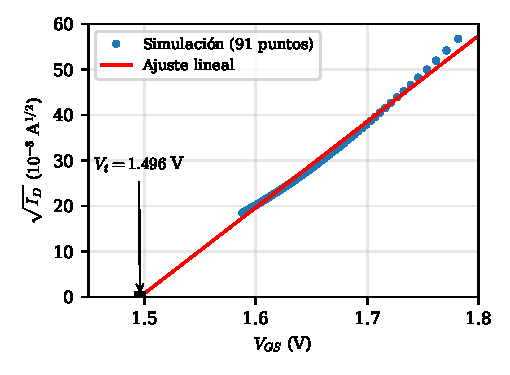
\includegraphics[width=0.68\columnwidth]{fig_sqrtid.pdf}
\caption{$\sqrt{I_D}$ en función de $V_{GS}$ obtenida variando $R_1$, con su ajuste lineal y el intercepto $V_t$.}
\label{fig:sqrtid}
\end{figure}

\subsection{Curvas características $I_D$--$V_{DS}$}
Con el circuito de la Fig.~\ref{fig:circ_car}(b) se hizo un barrido DC de $V_2$ de 0 a 10 V en pasos de 10 mV y $V_1$ de 2 a 4 V en pasos de 0.5 V. La Fig.~\ref{fig:curvas} muestra que cada curva sube en triodo y se vuelve horizontal en saturación.

\begin{figure}[htbp]
\centering
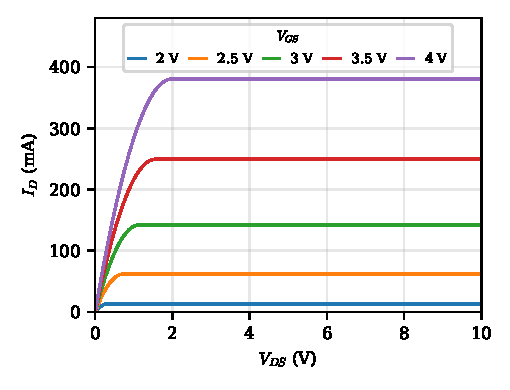
\includegraphics[width=0.68\columnwidth]{fig_curvas.pdf}
\caption{Curvas características $I_D$--$V_{DS}$ del MOSFET simulado para $V_{GS}$ de 2 a 4 V.}
\label{fig:curvas}
\end{figure}

\subsection{Amplificador de fuente común}
Se simuló el circuito de la Fig.~\ref{fig:cs} con los valores de la Tabla~\ref{tab:param_cs}, una fuente senoidal de 50 mV de amplitud a 10 kHz y un análisis transitorio de 500 $\mu$s. La Fig.~\ref{fig:trans} muestra las tensiones entre 300 y 500 $\mu$s. Ajustando senoides de 10 kHz entre 200 y 500 $\mu$s se obtienen amplitudes de \SI{50.00}{mV} (entrada) y \SI{247.7}{mV} (salida), un desfase de salida de $-174.9^\circ$, $A_v=-4.95$ V/V y, con un ajuste de armónicos, $HD_2=\SI{3.45}{\percent}$.

\begin{figure}[htbp]
\centering
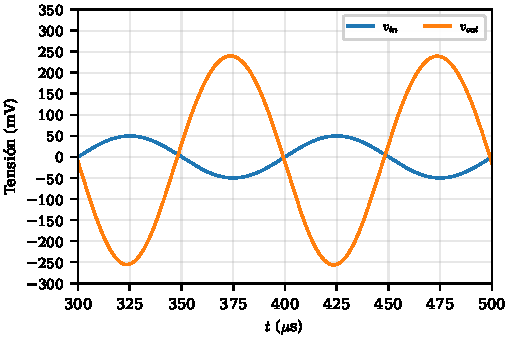
\includegraphics[width=0.92\columnwidth]{fig_transitoria.pdf}
\caption{Tensiones de entrada y de salida simuladas del amplificador de fuente común a 10 kHz.}
\label{fig:trans}
\end{figure}

%==================================================================
\section{Montaje}
%==================================================================
% (Sección pendiente hasta realizar el montaje en el laboratorio.)

%==================================================================
\section{Análisis de resultados}
%==================================================================

\subsection{Caracterización del MOSFET}
En la Fig.~\ref{fig:sqrtid} se observa que $\sqrt{I_D}$ crece de forma aproximadamente lineal con $V_{GS}$, como predice la \eqref{eq:raiz}, con $R^2=0.9932$; el intercepto $V_t=\SI{1.496}{V}$ está dentro del rango de la hoja de datos y el $\kn$ puntual difiere \SI{4.59}{\percent} del de la pendiente. El transistor permanece en saturación para cualquier $R_1$ porque $V_{DS}=V_{GS}>V_{GS}-V_t$; $R_1$ solo desplaza el punto sobre la curva según la \eqref{eq:kvl_car}. La relación es lineal porque en saturación $\sqrt{I_D}\propto V_{GS}-V_t$, y el intercepto es $V_t$ porque allí $\sqrt{I_D}=0$ y el canal deja de existir.

\subsection{Curvas características y parámetros de operación}
\label{sec:an_curvas}
En la Fig.~\ref{fig:curvas} es posible observar que la corriente de saturación crece con $V_{GS}$ y es casi independiente de $V_{DS}$ tras la frontera de la \eqref{eq:frontera}. Las curvas permiten ubicar el punto de operación y son específicas de cada ejemplar porque dependen de su $V_t$ y $\kn$. La Tabla~\ref{tab:isat} compara las corrientes simuladas con las de la \eqref{eq:sat} usando la \eqref{eq:param_op}.

\begin{table}[htbp]
\centering
\caption{Corriente de saturación simulada frente a la \eqref{eq:sat} con $\Vtp$ y $\knp$, y error relativo.}
\label{tab:isat}
\scriptsize
\renewcommand{\arraystretch}{1.05}
\begin{tabular}{@{}cccc@{}}
\toprule
$V_{GS}$ (V) & $I_D$ simulada (mA) & $I_D$ modelo (mA) & Error (\%) \\
\midrule
2.0 & 13.07 & 13.31 & 1.84 \\
2.5 & 61.93 & 60.88 & 1.70 \\
3.0 & 142.19 & 142.98 & 0.56 \\
3.5 & 249.41 & 259.61 & 4.09 \\
4.0 & 380.18 & 410.76 & 8.04 \\
\bottomrule
\end{tabular}
\end{table}

Con $\Vtp$ y $\knp$ el error es menor que \SI{2}{\percent} entre 2 y 3 V y llega a \SI{8.04}{\percent} en 4 V. Con los parámetros de la \eqref{eq:recta}, obtenidos cerca del umbral, la \eqref{eq:sat} subestima la corriente entre \SI{30.5}{\percent} y \SI{43.1}{\percent} en ese intervalo, porque la pendiente de $\sqrt{I_D}$ aumenta con $V_{GS}$ (de \SI{0.19}{A^{1/2}/V} cerca del umbral a \SI{0.26}{A^{1/2}/V} entre 2 y 3 V). Por eso $V_t$ y $\kn$ deben extraerse cerca de la zona de operación y el amplificador se diseña con $\Vtp$ y $\knp$. Además, para $V_{GS}\ge\SI{3.5}{V}$ la corriente supera los \SI{200}{mA} de la hoja de datos y en $V_{GS}=\SI{4}{V}$ la potencia llega a \SI{3.80}{W}, frente a $P_D=\SI{1}{W}$, por lo que el barrido de laboratorio debe restringirse.

\subsection{Amplificador de fuente común}
En la Fig.~\ref{fig:trans} es posible observar que la salida está invertida y que su amplitud es casi cinco veces la de la entrada; los picos son $+\SI{240.0}{mV}$ y $-\SI{256.6}{mV}$, asimetría debida al segundo armónico. La Tabla~\ref{tab:av} compara teoría y simulación.

\begin{table}[htbp]
\centering
\caption{Amplificador de fuente común: teoría frente a simulación.}
\label{tab:av}
\scriptsize
\renewcommand{\arraystretch}{1.05}
\begin{tabular}{@{}lccc@{}}
\toprule
Magnitud & Teoría & Simulación & Error (\%) \\
\midrule
$A_v$ (V/V) & $-4.86$ & $-4.95$ & 1.82 \\
Amplitud de $v_{out}$ (mV) & 243 & 247.7 & 1.90 \\
$\angle A_v$ ($^\circ$) & $-175.0$ & $-174.9$ & 0.06 \\
$HD_2$ (\%) & 3.17 & 3.45 & 8.12 \\
\bottomrule
\end{tabular}
\end{table}

El requisito $|v_{out}|\approx 5\,|v_{in}|$ se cumple en teoría y en simulación: $|A_v|=4.86$ se desvía \SI{2.8}{\percent} de 5 y $|A_v|=4.95$ se desvía \SI{0.9}{\percent}. La ganancia teórica y la simulada difieren \SI{1.82}{\percent}, lo que valida el uso de los parámetros de operación, y el desfase simulado coincide con el de la \eqref{eq:fase} (inversión con $5^\circ$ de adelanto por $C_S$, cuyo polo es el de la \eqref{eq:fc}). Las impedancias de la \eqref{eq:zin_zout} no dependen de $\kn$ ni de $V_t$. El $HD_2$ simulado es algo mayor que el teórico porque la \eqref{eq:limite} solo usa el modelo cuadrático, pero ambos son menores que \SI{5}{\percent} y la entrada de 50 mV es menor que el límite de \SI{79}{mV}. Además, el transistor sigue en saturación ($V_{DS}=\SI{7.42}{V}\ge\Vov=\SI{0.40}{V}$) y $|A_v|>1$, condiciones básicas para que haya amplificación.

% --- Comparación con mediciones de laboratorio (completar tras el montaje) ---
% \subsection{Comparación con las mediciones}

%==================================================================
\section{Conclusiones}
%==================================================================
\begin{enumerate}
\item El ajuste de $\sqrt{I_D}$ contra $V_{GS}$ dio $V_t=\SI{1.496}{V}$, dentro del intervalo de la hoja de datos (0.8 a 3 V), y $\kn=\SI{71.52}{mA/V^2}$; el cálculo puntual difiere \SI{4.59}{\percent} del ajuste.
\item Con la compuerta unida al drenador el transistor permanece en saturación para cualquier $R_1$, lo que explica la linealidad de $\sqrt{I_D}$ y que $V_t$ sea el intercepto.
\item Los parámetros extraídos cerca del umbral subestiman $I_D$ entre \SI{30.5}{\percent} y \SI{43.1}{\percent} en $V_{GS}$ de 2 a 4 V; con $\Vtp=\SI{1.561}{V}$ y $\knp=\SI{138.1}{mA/V^2}$ el error es menor que \SI{2}{\percent} entre 2 y 3 V y de \SI{8.04}{\percent} en 4 V, por lo que el modelo cuadrático es válido solo localmente.
\item El amplificador queda polarizado en saturación ($I_D=\SI{10.77}{mA}$, $V_{DS}=\SI{7.42}{V}$), con $Z_{in}=\SI{64.29}{k\ohm}$ y $Z_{out}=\SI{90}{\ohm}$, y la ganancia teórica ($-4.86$) difiere \SI{1.82}{\percent} de la simulada ($-4.95$): ambas cumplen $\vert{}v_{out}\vert{}\approx 5\,\vert{}v_{in}\vert{}$ (desviaciones de \SI{2.8}{\percent} y \SI{0.9}{\percent}) y su fase coincide ($-175.0^\circ$ frente a $-174.9^\circ$).
\item La entrada de 50 mV queda por debajo del límite de pequeña señal de \SI{79}{mV}, con $HD_2$ de \SI{3.17}{\percent} teórico y \SI{3.45}{\percent} simulado, ambos menores que \SI{5}{\percent}.
% \item (Conclusión comparativa teoría--simulación--medición: completar tras el montaje.)
\end{enumerate}

%==================================================================
\begin{thebibliography}{6}
\bibitem{sedra} A. S. Sedra, K. C. Smith, T. C. Carusone, and V. Gaudet, \emph{Microelectronic Circuits}, 8th ed. New York, NY, USA: Oxford Univ. Press, 2020.

\bibitem{datasheet} Microchip Technology Inc., ``2N7000: N-channel enhancement-mode vertical DMOS FET,'' Datasheet DS20005695A, 2021. [Online]. Available: \url{https://static.chipdip.ru/lib/597/DOC011597112.pdf}

\bibitem{shea} P. Shea, ``Design and modeling of radiation hardened LDMOSFET for spacecraft power systems,'' M.S.E.E. thesis, Univ. of Central Florida, Orlando, FL, USA, 2007. [Online]. Available: \url{https://stars.library.ucf.edu/etd/3344}

\bibitem{lauenstein} J.-M. Lauenstein, ``Challenges for radiation hardness assurance (RHA) on power MOSFETs,'' presented at the NEPP Electronic Technology Workshop, NASA Goddard Space Flight Center, Greenbelt, MD, USA, 2012. [Online]. Available: \url{https://ntrs.nasa.gov/api/citations/20120014270/downloads/20120014270.pdf}

\bibitem{kao} S.-T. Kao and C.-C. Su, ``A 0.8-V low power analog front-end IC for biomedical signal recording,'' thesis, Inst. Elect. Control Eng., Nat. Chiao Tung Univ., Hsinchu, Taiwan, 2008. [Online]. Available: \url{http://hdl.handle.net/11536/41083}

\bibitem{litwin} A. Litwin, Q. Chen, J. Johansson, G. Ma, L.-A. Olofsson, and P. Perugupalli, ``High power LDMOS technology for wireless infrastructure,'' in \emph{Proc. GaAs Applications Symp. (GAAS 2001)}, London, U.K., Sep. 2001. [Online]. Available: \url{https://amsacta.unibo.it/id/eprint/65/}
\end{thebibliography}

\end{document}